\documentclass[12pt,a4paper]{article}
\usepackage[utf8]{vietnam}
\usepackage{amsmath,amssymb}
\usepackage{tabularx}
\usepackage{tikz}
\usetikzlibrary{calc,angles,quotes,arrows.meta,patterns}
\usepackage{xcolor}
\usepackage{enumitem}
\usepackage{fancyhdr}
\usepackage[top=1.2cm, bottom=1.2cm, left=1.5cm, right=1.5cm]{geometry}
\usepackage[dethi]{ex_test}
\SAOPTN{widthSA=2.6,heightSA=0.62}

\setlength{\headheight}{15pt}
\setlength{\parskip}{0pt}

% Dòng kẻ chấm mờ chuẩn viết tay
\newcommand{\dongke}[1]{%
  \begingroup%
  \setlength{\parskip}{0pt}%
  \baselineskip=18.5pt%
  \vspace{1.0mm}%
  \foreach \i in {1,...,#1}{%
    \noindent{\color{gray!60}\dotfill}\par%
  }%
  \vspace{0.6mm}%
  \endgroup%
}

\pagestyle{fancy}
\fancyhf{}
\rhead{\textit{Môn Toán 6 -- Đề số 1}}
\lhead{\textit{Bộ đề ôn tập Giữa học kì I}}
\cfoot{\thepage}

\begin{document}

% --- KHUNG TIÊU ĐỀ ĐỀ THI ---
\noindent
\begin{tabularx}{\linewidth}{X r}
\textbf{TRƯỜNG THCS: \dotfill} & \textbf{ĐỀ KIỂM TRA ĐỊNH KỲ GIỮA HỌC KỲ I} \\
\textbf{Họ và tên: \dotfill} & \textbf{NĂM HỌC 2026 -- 2027} \\
\textbf{Lớp: \dotfill \quad SBD: \dotfill} & \textbf{Môn: TOÁN 6} \\
\hline
\end{tabularx}
\vspace{2mm}

\begin{center}
  \textbf{\large ĐỀ ÔN TẬP GIỮA HỌC KỲ I -- ĐỀ SỐ 1}\\
  \textit{Thời gian làm bài: 90 phút (Không kể thời gian phát đề)}
\end{center}
\vspace{1mm}

% --- PHẦN I ---
\noindent\textbf{\large PHẦN I. CÂU TRẮC NGHIỆM NHIỀU PHƯƠNG ÁN LỰA CHỌN (3,0 điểm)}

\textit{Thí sinh trả lời từ câu 1 đến câu 12. Mỗi câu hỏi thí sinh chỉ chọn một phương án duy nhất.}

\vspace{1mm}
\begin{ex}
Tập hợp nào dưới đây là tập hợp số tự nhiên?
\choice
{$\mathbb{N} = \{1; 2; 3; \dots\}$}
{$\mathbb{N} = \{0; 1; 2; 3; \dots; 100\}$}
{\True $\mathbb{N} = \{0; 1; 2; 3; \dots\}$}
{$\mathbb{N} = \{0; 2; 4; 6; \dots\}$}
\end{ex}

\begin{ex}
Với $a, m, n$ là các số tự nhiên, khẳng định nào sau đây là đúng?
\choice
{\True $a^m : a^n = a^{m-n}$ ($a \neq 0, m \geq n$)}
{$a^m : a^n = a^{m+n}$ ($a \neq 0$)}
{$a^m \cdot a^n = a^{m:n}$ ($a \neq 0$)}
{$a^m : a^n = m - n$ ($a \neq 0$)}
\end{ex}

\begin{ex}
Thứ tự thực hiện phép tính nào sau đây là đúng đối với biểu thức không có dấu ngoặc?
\choice
{Nhân và chia $\to$ Lũy thừa $\to$ Cộng và trừ}
{Cộng và trừ $\to$ Nhân và chia $\to$ Lũy thừa}
{\True Lũy thừa $\to$ Nhân và chia $\to$ Cộng và trừ}
{Cộng và trừ $\to$ Lũy thừa $\to$ Nhân và chia}
\end{ex}

\begin{ex}
Hình vuông $ABCD$ có cạnh $AB = 3\text{ cm}$. Diện tích của hình vuông đó là:
\choice
{$3\text{ cm}^2$}
{\True $9\text{ cm}^2$}
{$12\text{ cm}^2$}
{$81\text{ cm}^2$}
\end{ex}

\begin{ex}
Số $19$ trong hệ La Mã được viết là:
\choice
{IX}
{IXX}
{XXI}
{\True XIX}
\end{ex}

\begin{ex}
Trong các phân số sau, phân số nào là phân số tối giản?
\choice
{$\dfrac{26}{39}$}
{$\dfrac{15}{12}$}
{$\dfrac{27}{42}$}
{\True $\dfrac{3}{16}$}
\end{ex}

\begin{ex}
Tập hợp các chữ cái trong cụm từ “PHONG NHA” là:
\choice
{$\{P; H; O; N; G; N; H; A\}$}
{\True $\{P; H; O; N; G; A\}$}
{$\{H; O; N; G; P; A\}$}
{$\{N; A; P; O; G\}$}
\end{ex}

\begin{ex}
Trong các số sau, số nào là bội của $7$?
\choice
{$15$}
{$20$}
{$25$}
{\True $35$}
\end{ex}

\begin{ex}
Thực hiện phép tính $3^2 + 3^3$ được kết quả là:
\choice
{$45$}
{\True $36$}
{$432$}
{$423$}
\end{ex}

\begin{ex}
\immini{
Từ hình bên có bao nhiêu hình vuông?
\choice
{$4$ hình vuông}
{\True $5$ hình vuông}
{$6$ hình vuông}
{$8$ hình vuông}
}{
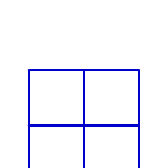
\begin{tikzpicture}[scale=0.7, baseline=(current bounding box.center), line cap=round, line join=round]
  \draw[step=1cm, thick, blue!80!black] (0,0) grid (2,2);
\end{tikzpicture}
}
\end{ex}

\begin{ex}
Tập hợp tất cả các ước của số $20$ là:
\choice
{\True $\text{Ư}(20) = \{1; 2; 4; 5; 10; 20\}$}
{$\text{Ư}(20) = \{0; 1; 2; 4; 5; 10\}$}
{$\text{Ư}(20) = \{1; 2; 5; 10\}$}
{$\text{Ư}(20) = \{1; 2; 10; 20\}$}
\end{ex}

\begin{ex}
Ghép $6$ tam giác đều có độ dài cạnh $3\text{ cm}$ thành một lục giác đều. Khi đó độ dài đường chéo chính của lục giác đều là:
\choice
{$9\text{ cm}$}
{$3\text{ cm}$}
{$12\text{ cm}$}
{\True $6\text{ cm}$}
\end{ex}


\vspace{1mm}
\noindent\textbf{BẢNG TRẢ LỜI TRẮC NGHIỆM PHẦN I:}
\begin{center}
\begin{tabular}{|c|c|c|c|c|c|c|c|c|c|c|c|c|}
\hline
\textbf{Câu} & \textbf{1} & \textbf{2} & \textbf{3} & \textbf{4} & \textbf{5} & \textbf{6} & \textbf{7} & \textbf{8} & \textbf{9} & \textbf{10} & \textbf{11} & \textbf{12} \\
\hline
\textbf{Chọn} & \rule{0pt}{0.65cm} & & & & & & & & & & & \\
\hline
\end{tabular}
\end{center}
\vspace{2mm}

\setcounter{ex}{0}
\noindent\textbf{\large PHẦN II. CÂU TRẮC NGHIỆM ĐÚNG SAI (2,0 điểm)}

\textit{Thí sinh trả lời câu 1 và câu 2. Trong mỗi ý a), b), c), d) ở mỗi câu, thí sinh chọn đúng hoặc sai.}

\vspace{1mm}
\begin{ex}
Cho $N$ là tập hợp các số tự nhiên chẵn nhỏ hơn $10$. Các khẳng định sau đây đúng hay sai?
\choiceTF
{\True Tập hợp $N$ được viết theo cách liệt kê các phần tử là $N = \{0; 2; 4; 6; 8\}$}
{\True Số phần tử của tập hợp $N$ là $5$ phần tử}
{Số $10$ thuộc tập hợp $N$ (kí hiệu $10 \in N$)}
{Tập hợp $N$ có thể được viết bằng cách chỉ ra tính chất đặc trưng là $N = \{x \in \mathbb{N} \mid x \text{ là số chẵn}\}$}
\end{ex}

\begin{ex}
Cho hình chữ nhật $ABCD$ có độ dài cạnh $AB = 5\text{ cm}$ và $BC = 2\text{ cm}$. Các khẳng định sau đây đúng hay sai?
\choiceTF
{\True Độ dài cạnh $CD = 5\text{ cm}$ và độ dài cạnh $AD = 2\text{ cm}$}
{\True Chu vi của hình chữ nhật $ABCD$ bằng $14\text{ cm}$}
{\True Diện tích của hình chữ nhật $ABCD$ bằng $10\text{ cm}^2$}
{\True Hình chữ nhật $ABCD$ có $2$ trục đối xứng}
\end{ex}


\noindent\textbf{BẢNG TRẢ LỜI PHẦN II:}
\begin{center}
\begin{tabular}{|c|c|c|c|c||c|c|c|c|c|}
\hline
\textbf{Câu 1} & \textbf{a)} & \textbf{b)} & \textbf{c)} & \textbf{d)} & \textbf{Câu 2} & \textbf{a)} & \textbf{b)} & \textbf{c)} & \textbf{d)} \\
\hline
\textbf{Đ/S} & \rule{0pt}{0.6cm} & & & & \textbf{Đ/S} & & & & \\
\hline
\end{tabular}
\end{center}
\vspace{2mm}

\setcounter{ex}{0}
\noindent\textbf{\large PHẦN III. CÂU HỎI TRẢ LỜI NGẮN (2,0 điểm)}

\textit{Thí sinh trả lời câu 1 và câu 2. Điền kết quả số vào ô trống tương ứng.}

\vspace{1mm}
\begin{ex}
Số liền trước của số nguyên tố nhỏ nhất là số mấy? \shortans{$1$}
\end{ex}

\begin{ex}
Mẹ Minh mua một túi gạo $15\text{ kg}$ loại $20\,000$ đồng mỗi $1\text{ kg}$. Hỏi mẹ Minh phải đưa cô bán hàng bao nhiêu tờ tiền loại $50\,000$ đồng để vừa đủ thanh toán tiền mua gạo trên? \shortans{$6$}
\end{ex}


\setcounter{ex}{0}
\noindent\textbf{\large PHẦN IV. TỰ LUẬN (3,0 điểm)}

\textit{Thí sinh trình bày chi tiết lời giải vào giấy làm bài.}

\vspace{1mm}
\begin{ex} (1.0 điểm)
Thực hiện phép tính (tính hợp lí nếu có thể):
\begin{enumerate}[label=\textbf{\alph*)}, leftmargin=0.8cm, itemsep=2pt]
\item $36 + 75 + 64 + 25 + 99$
\item $2024^0 + 3 \cdot [5^2 \cdot 10 - (23 - 13)^2]$
\item $4^2 \cdot 65 + 35 \cdot 4^2 - 1500$
\end{enumerate}
\end{ex}
\vspace{1.5mm}

\begin{ex} (0.75 điểm)
Một mảnh vườn hình chữ nhật có chiều dài $42\text{ m}$ và chiều rộng $30\text{ m}$.
\begin{enumerate}[label=\textbf{\alph*)}, leftmargin=0.8cm, itemsep=2pt]
\item Tính chu vi và diện tích của mảnh vườn.
\item Biết rằng mỗi túi hạt giống gieo vừa đủ $105\text{ m}^2$ đất và mỗi túi hạt giống có giá $45\,000$ đồng. Hỏi cần bao nhiêu túi hạt giống để gieo vừa hết mảnh vườn và cần bao nhiêu tiền để mua số túi hạt giống đó?
\end{enumerate}
\end{ex}
\vspace{1.5mm}

\begin{ex} (0.75 điểm)
\begin{enumerate}[label=\textbf{\alph*)}, leftmargin=0.8cm, itemsep=2pt]
\item[\textbf{1)}] Vẽ hình chữ nhật $ABCD$ biết cạnh $AB = 5\text{ cm}$ và cạnh $BC = 3\text{ cm}$.
\item[\textbf{2)}] Một khoảng sân có dạng hình chữ nhật với chiều dài $9\text{ m}$ và chiều rộng $4\text{ m}$. Người ta dành một phần của sân để trồng hoa (phần kẻ sọc trong hình bên), phần còn lại dùng để lát gạch (phần màu trắng).\
\begin{center}
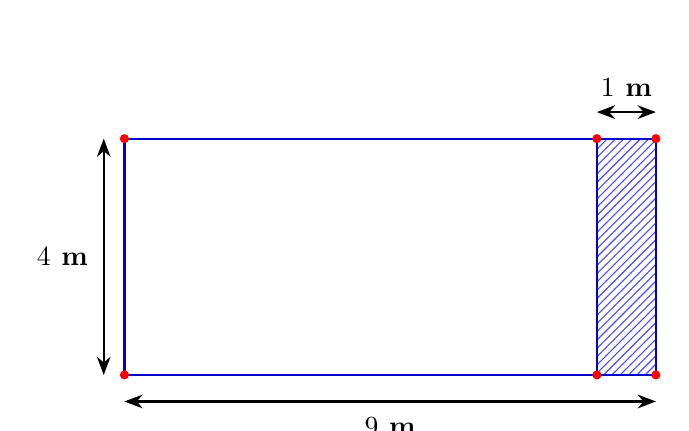
\begin{tikzpicture}[scale=0.75, line cap=round, line join=round, >=Stealth]
  \coordinate (A) at (0,4); \coordinate (B) at (9,4); \coordinate (C) at (9,0); \coordinate (D) at (0,0);
  \coordinate (E) at (8,4); \coordinate (F) at (8,0);
  \fill[pattern=north east lines, pattern color=blue!70] (E) rectangle (C);
  \draw[thick, blue!80!black] (D) rectangle (B);
  \draw[thick, blue!80!black] (E) -- (F);
  \foreach \p in {A,B,C,D,E,F} \fill[red] (\p) circle (2.2pt);
  \draw[<->, thick] (-0.35,0) -- (-0.35,4) node[midway, left=2pt, font=\bfseries] {$4\text{ m}$};
  \draw[<->, thick] (0,-0.45) -- (9,-0.45) node[midway, below=2pt, font=\bfseries] {$9\text{ m}$};
  \draw[<->, thick] (8,4.45) -- (9,4.45) node[midway, above=2pt, font=\bfseries] {$1\text{ m}$};
\end{tikzpicture}
\end{center}\
a) Tính diện tích phần sân dùng để trồng hoa.\
b) Nếu lát phần sân còn lại bằng những viên gạch hình vuông cạnh $40\text{ cm}$ thì cần bao nhiêu viên gạch? (Coi diện tích mạch ghép giữa các viên gạch là không đáng kể).
\end{enumerate}
\end{ex}
\vspace{1.5mm}

\begin{ex} (0.5 điểm)
\begin{enumerate}[label=\textbf{\alph*)}, leftmargin=0.8cm, itemsep=2pt]
\item Tính tổng $C = 1 + 3 + 3^2 + 3^3 + 3^4 + \dots + 3^{2020}$.
\item Tìm số tự nhiên $n$ sao cho $p = (n - 2)(n^2 + n - 5)$ là một số nguyên tố.
\end{enumerate}
\end{ex}
\vspace{1.5mm}


\begin{center}
\rule{4cm}{0.4pt}\\
\textit{--- HẾT ---}
\end{center}
\end{document}
